\begin{center}
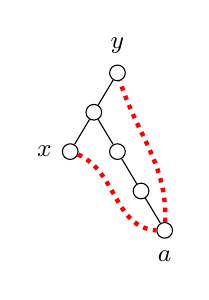
\begin{tikzpicture}[scale=.5,level distance=10mm, state/.style={circle, draw, minimum size=1mm}]]
  \tikzstyle{every node}=[font=\small, draw=black,circle,inner sep=2pt, minimum size=1mm]
  \tikzstyle{level 1}=[sibling distance=12mm, set style={{every node}+=[draw=black]}]
  \tikzstyle{level 2}=[sibling distance=12mm, set style={{every node}+=[draw=black]}]
  \tikzstyle{level 3}=[sibling distance=12mm,  set style={{every node}+=[draw=black]}]
  \tikzstyle{level 4}=[sibling distance=12mm,  set style={{every node}+=[draw=black]}]
  \tikzstyle{level 5}=[sibling distance=12mm,  set style={{every node}+=[draw=black]}]

    \node [label=above:{$y$}] (y) {}
     child {
        node {}
              child {node (x)[label=left:{$x$}] {}}
                child {node {}
                child[fill=none] {edge from parent[draw=none]}
                child {node {}
                child[fill=none] {edge from parent[draw=none]}
                child {node[label=below:{$a$}] (a) {}}}
                }
            }
    child[fill=none] {edge from parent[draw=none]};
    
    \draw[-,dotted,ultra thick,relative,red] (x) to[out=20,in=220] (a);
    
    \draw[-,dotted,ultra thick,relative,red] (a) to[out=-20,in=180] (y);
       
\end{tikzpicture}
\end{center}